\section{Correlated velocity uncertainty through a fixed survey estimator}
A velocity-field model becomes relevant to the apparent expansion
coefficients only after it is propagated through the same estimator that
produced them. Freeze the catalogue distances, directions, weights and
row order, and write

\[
 \widehat\theta=A y,\qquad y_i=c z_{{\rm CMB},i},\qquad
 A_w=(X_w^T W_wX_w)^{-1}X_w^T W_w,
 \quad X_{w,i}=d_i(1,n_i,E_1:n_in_i,\ldots,E_5:n_in_i).
\]

The four window blocks form a 36 by 35,970 operator. The directions are
outward ICRS J2000, distances are in Mpc, the input is in km/s, and the
output coefficients are in km/s/Mpc. The released redshift defines a
fixed proxy; it is not varied as an observer parameter. The five
matrices \(E_A\) form the signed orthonormal STF basis used earlier.
Applying the same operator to a source bulk velocity and to observer
motion gives \([AN,-AN]\), where row \(i\) of \(N\) is \(n_i^T\).
Consequently \((h,h)\) is a null direction for every constant vector
\(h\). This statement concerns source minus observer velocity; the
earlier comparison between a velocity response and a constant
apparent-rate dipole is a different design comparison.

For an independent source-error component with diagonal variance \(D\),
a common velocity-field factor \(V\), and mean-design offsets \(Z\eta\)
with covariance \(\Sigma\), the propagated covariance is

\[
 C_\theta=A\operatorname{diag}(D)A^T+(AV)(AV)^T+K\Sigma K^T,
 \qquad K=AZ.
\]

Independence is part of this stipulated decomposition. Correlated source
classes require their joint factors and cross terms. The original
weighting law, \(250^2+[70(\ln10/5)d_i e_{{\rm DM},i}]^2\), already
contains a velocity-scale term and has no established empirical
decomposition. We display its propagated working covariance separately.
It is neither added to nor subtracted from the new conditional total.

The velocity calculation uses the Eisenstein--Hu no-wiggle approximation
and a common present-day Gaussian density realization, propagated with
the prescribed linear growth factors. The numerical background is
\(H_0=67.36\) km/s/Mpc, \(\Omega_m=0.3153\), \(\Omega_\Lambda=0.6847\),
\(\omega_b=0.02237\), \(n_s=0.9649\), and \(\sigma_8=0.8111\). The two
wavenumber bands are \([0.005,0.02]\) and
\([0.02,0.05]\,h\,{\rm Mpc}^{-1}\), with \(h=0.6736\). Shared Gaussian
smoothing radii are 5, 10 and 20 \(h^{-1}\) Mpc. At a positive
quadrature node, the source response is proportional to

\[
 b_i(k,\hat k)=g_i(n_i\!\cdot\!\hat k)e^{ik\hat k\cdot x_i}
 \left[\frac{P_0(k)w_k w_\Omega}{(2\pi)^3}\right]^{1/2} S_R(k),
 \qquad x_i=\chi(z_{{\rm CMB},i})n_i,
 \quad g_i=a_iH_if_iD_i.
\]

Real and imaginary projected columns give a positive-semidefinite Gram
matrix. There is no magnitude derivative in this velocity-to-rate
response. All radii and windows see the same field, yielding a full
108-coordinate covariance rather than independent blocks.

\begin{table}[htbp]
\centering\small
\caption{Propagated covariance traces in $(\mathrm{km/s/Mpc})^2$. Each band/radius row is its 36-coordinate block; inherited working covariance is separate from the stipulated total.}\label{tab:cf4cov}
\begin{tabular}{lll}
\toprule
Component & $R\;(h^{-1}\mathrm{Mpc})$ & Trace \\
\midrule
1 & 5 & 8.97773049 \\
1 & 10 & 8.85792223 \\
1 & 20 & 8.39976465 \\
2 & 5 & 8.08061983 \\
2 & 10 & 7.50105206 \\
2 & 20 & 5.65204638 \\
Combined PV & 5 & 17.05835032 \\
Inherited working & 5 & 4.76965546 \\
Stipulated total & 5 & 17.68057386 \\
\bottomrule
\end{tabular}
\end{table}

At 5 \(h^{-1}\) Mpc the two band traces sum to 17.05835032
\((\mathrm{km/s/Mpc})^2\). The original working trace is 4.76965546 in
these units. A separate total, which stipulates an independent 150 km/s
source term and four independent method mean-design offsets with
standard deviation 0.4 km/s/Mpc, has trace 17.68057386. The offsets use
\(Z_{im}=d_i1_{m(i)=m}\); this is not a magnitude-zero-point derivative.
Varying the distance calibration itself would also change distances,
design and possibly weights. Power outside the two bands, nonlinear
velocities, the empirical source-selection law and calibration/PV cross
terms are not supplied by this calculation.

\begin{figure}[htbp]
\centering
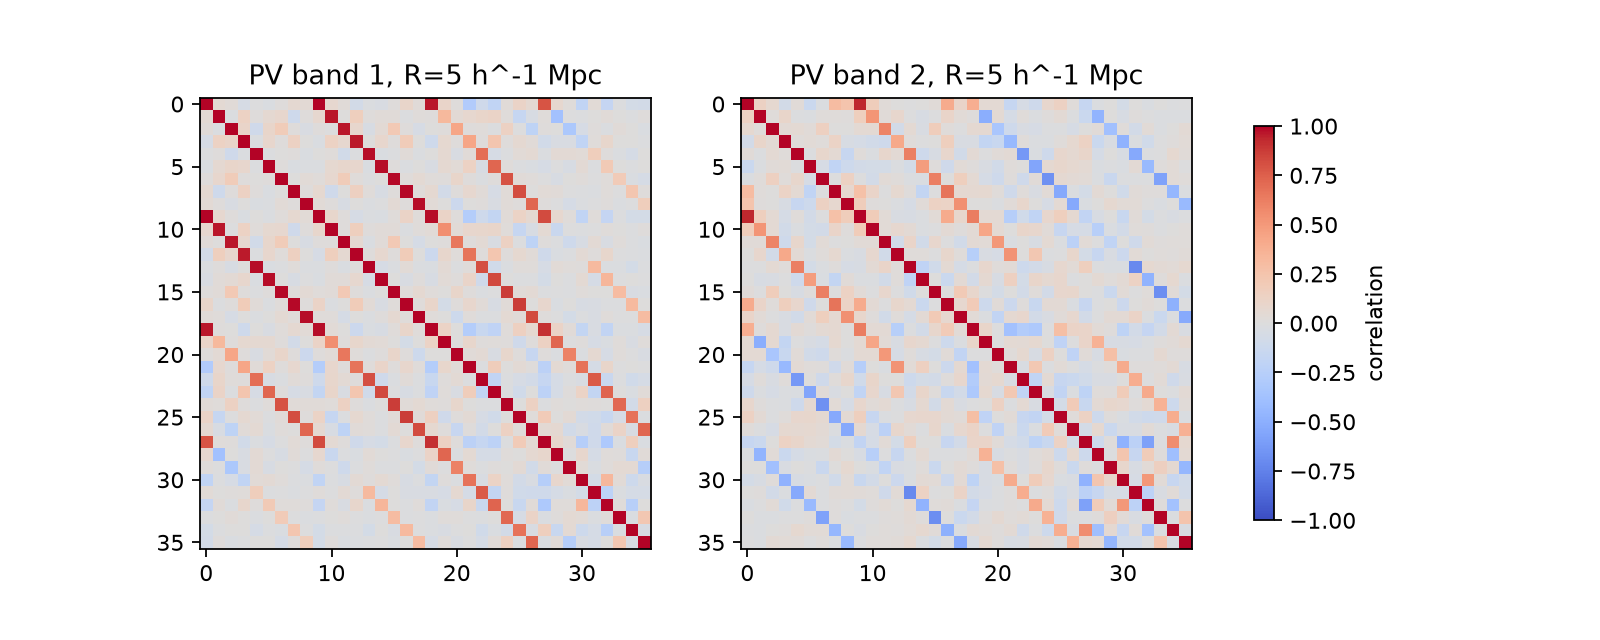
\includegraphics[width=0.95\linewidth]{r36_bridge/cf4_correlation.png}
\caption{Correlation of the propagated apparent coefficients for the two prescribed velocity bands at R=5 $h^{-1}$ Mpc. Each consecutive block of nine coordinates contains a monopole, three signed dipole components and five STF components in one redshift window. The off-diagonal blocks retain the common-source velocity field. These matrices describe the conditional Gaussian band model; they are not estimates of the complete empirical survey covariance.}
\end{figure}

\begin{table}[htbp]
\centering\small
\caption{PV trace ratios relative to the full sample at the same radius. Subsets overlap.}\label{tab:footprint}
\begin{tabular}{lllll}
\toprule
Subset & Groups & $R=5$ & $R=10$ & $R=20$ \\
\midrule
exclude\_FP & 9054 & 1.172665 & 1.172335 & 1.171046 \\
exclude\_TF & 28356 & 0.867055 & 0.866170 & 0.863461 \\
north\_ICRS\_nz\_nonnegative & 27800 & 2.404822 & 2.353335 & 2.171901 \\
south\_ICRS\_nz\_negative & 8170 & 2.580425 & 2.531798 & 2.360402 \\
\bottomrule
\end{tabular}
\end{table}

Removing or restricting catalogue subsets changes the response even
under the same field model. At the smallest radius, northern and
southern ICRS subsets have PV trace ratios 2.405 and 2.580 relative to
the full sample; removing FP or TF groups gives 1.173 and 0.867. The
corresponding ratios at the largest radius are 2.172, 2.360, 1.171 and
0.863. These are overlapping-source, footprint-dependent estimator
comparisons. They provide a quantitative reason to retain the actual
survey support, rather than independent confirmations of an anisotropic
flow.

Under the stipulated 36-coordinate total covariance at the smallest
radius, a prespecified comparison of a shared monopole, affine monopole
and shared nine-coordinate mean gives minimum discrepancies 174.925896,
145.158891 and 80.137690, with ranks 1, 2 and 9. The rule
\(T+\operatorname{rank}\ln36\) selects the nine-coordinate mean. The
retained 2,000-draw Gaussian selected-statistic reference under the
fitted shared-monopole model gives an upper-tail estimate
\(1/2001=0.00049975\), with Monte Carlo standard error approximately
0.00050. This is a finite check of that stipulated reference. It is not
an empirical CF4 population probability, and it is not directly
comparable to the earlier 12-coordinate dipole statistic, which uses a
different response and covariance. A sample-covariance inverse
correction alone would not validate a selected statistic; for example,
the Gaussian 64-mock, 36-coordinate inverse factor \(26/63\) leaves
finite-covariance uncertainty to be propagated.
